\documentclass[a4paper,11pt,twocolumn,twoside]{article}
\usepackage{graphicx}
\usepackage{sepln_en}
\usepackage{fullname}
\usepackage[utf8]{inputenc}
\usepackage{booktabs}
\usepackage{tabularx}
\usepackage{todonotes}
% \usepackage[spanish,es-nosectiondot, es-tabla, es-noindentfirst, es-nolists]{babel}

\input epsf

\setlength\titlebox{4in} %esto por defecto

\title{Overview of the eHealth Knowledge Discovery Challenge at IberLEF 2021}

\author {\textbf{Nombre Apellidos1,$^1$} \textbf{Nombre Apellidos2$^2$}\\
$^1$Universidad o lugar de trabajo\\
$^2$Universidad o lugar de trabajo\\
Información de contacto\\
}

\seplntranstitle{Resumen de la Tarea de Descubrimiento de Conocimiento en Salud en IberLEF 2021}

\seplnclave{Palabras, palabras, palabras en castellano...}

\seplnresumen{Resumen del artículo en castellano con una sangría a izquierda y
derecha de 1 cm, justificado por ambos lados, con tamaño de fuente
11.}


\seplnkey{Palabras, palabras, palabras en inglés...}

\seplnabstract{Resumen del artículo en inglés con una sangría a izquierda y
derecha de 1 cm, justificado por ambos lados, con tamaño de fuente
11.}

\firstpageno{1}

\begin{document}

% la siguiente instrucción sólo se debe usar si el abstract sobrescribe el texto
% la longitud variará según se necesite

%\setlength\titlebox{20cm} % se aumenta el tamaño del espacio reservado para datos de título

\label{firstpage} \maketitle

%\begin{abstract}
%Resumen del artículo con una sangría a izquierda y derecha de 0.32
%cm, justificado por ambos lados, con tamaño de fuente 11.
%
%\end{abstract}

\section{Introduction}


The accelerated growth of the Internet and the increased production of textual resources in all areas of human endeavour has created both new opportunities and new challenges for the research community.
On one hand, larger datasets can be collected and used to build increasingly powerful machine learning models~(e.g., GPT-3 and related).
On the other hand, is becoming increasingly difficult to organise, categorise, cross-reference, and fact-check the textual information available online.
The ease of access to both publication and consumption of textual information is arguably one of the root causes of the increasingly worrying phenomenon of fake news.

Staying up-to-date on information about topics of interest is crucial in technical or scientific domains.
For this purpose, specialists rely on a combination of curated soruces (e.g., domain-specific repositories like arxiv, bioarxiv, semantic scholar) and technologies for search and recommendation (e.g., google scholar).
These resources significantly improve the experience of collecting and consuming large amounts of relevant information on a specific topic.
Tools like Connected Papers~\cite{} and Papers with Code~\cite{} are one step beyond the indexing of documents, providing summarised and structured representations of the content in a collection of documents.
However, it remains an open problem to automatically combine, summarise, and present the relevant information in a collection of documents in a semantic structure~(e.g., a knowledge graph) that allows a specialist to quickly grasp the essential concepts of a specific knowledge field.

A potential solution to this problem would require methods to automatically detect in natural language the most relevant concepts and the factual statements in which they are related, possibly normalise them into well-established taxonomies and classifications, and store them in computational data structures where they can linked with related concepts, e.g., knowledge graphs.
The first step of this process, i.e., the detection of relevant concepts and semantic relations in text, is already a challenging computational task, given the complexity and variability of natural language.
To encourage research and development in this area, several academic competitions have been organised through the years by organizations such as CLEF, SEMEVAL, and more recently, IBERLEF.

In this context, the eHealth Knowledge Discovery Challenge is designed to foster the development of automatic knowledge discovery systems for natural language sentences in a cross-domain and multi-lingual setting.
Concretely, a token-level annotation model of 4 entities and 13 semantic relations is defined, and a corpus of more than 1500 sentences from different factual sources~(i.e., Spanish Medline articles, Spanish Wikinews articles, and English biomedical preprints related to COVID-19) is annotated.
Two computational tasks are defined: the detection of multi-span, non-contiguous, and potentially overlapping named entities; and the detection of semantic relations between them.
A shared annotation campaign was organized, where a total of 9 participants presented 10 different systems with varied levels of performance.

The eHealth-KD task focuses on cross-domain, multi-lingual and low-resource solutions. This setting presents a significant challenge to existing state-of-the-art methods, which often rely on large amounts of training data.
A succesful approach to the eHealth-KD must leverage transfer learning across different domains and languages, since the vast majority of the training examples are provided in Spanish language and from the Medline domain, while only a small development set is available in the remaining settings.
With this added complexity, we expect to encourage solutions that can be deployed in low-resource environments, where is unfeasible to train large language models over longs periods of time.

The remaining of this paper is organized as follows.
Section~\ref{sec:task} describes the eHealth-KD tasks in greater detail, including the annotation model and performance metrics.
Section~\ref{sec:resources} describes the corpora and other resources created for this challenge and presents some qualitative analysis of their characteristics.
Section~\ref{sec:systems} describes the different systems presented in the challenge and summarises the main approaches and most common characteristics they share.
Section~\ref{sec:results} presents the main results of the challenge.
Section~\ref{sec:discussion} discusses the most interesting insights of the challenge and highlights both the most relevant lessons learned and potential improvements for future similar endeavours.

\section{Tasks Descriptions}\label{sec:task}

\begin{figure*}[htb]
  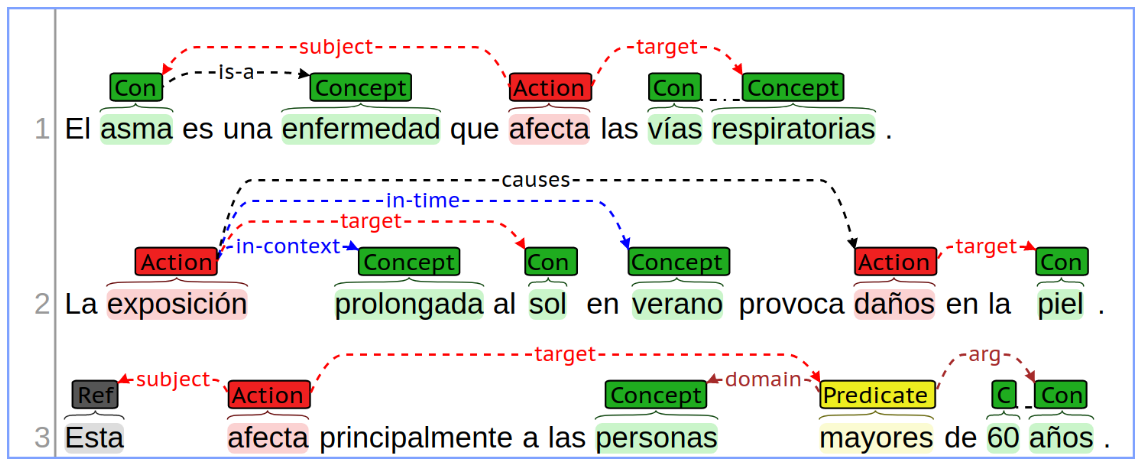
\includegraphics[width=\textwidth]{model.png}
  \caption{Examples the annotation model defined for the eHealth-KD Challenge.\label{fig:model}}
\end{figure*}

The eHealth-KD challenge consists on the automatic sentence-level annotation
of multi-token entities and binary relations among them.
A custom annotation model has been defined, comprising 4 entity types and 13 relations,
that attempts to capture a large part of factual semantics in technical documents,
including enciclopedias, news, and scientific papers. The annotation model is explained in detail in \namecite{piad2019general}. Figure~\ref{fig:model} shows an illustrative example of the annotation model in three Spanish sentences.
The challenge has been divided into two different subtasks: entity recognition and relation extraction.

\subsection{Subtask A: Entity recognition}

The goal of this subtask is to identify all the entities per document and their types. These entities are all the relevant terms (single word or multiple words) that represent semantically important elements in a sentence. Entities always consist of one or more complete words (i.e., not a prefix or a suffix of a word), and never include any surrounding punctuation symbols, parenthesis, etc. There are four types for entities:

\begin{description}
  \item[Concept:] indentifies a rel willevant term, concept, idea, in the knowledge domain of the sentence.
  \item[Action:] indentifies a process or modification of other entities. It can be indicated by a verb or verbal construction, such as “afecta” (affects), but also by nouns, such as “exposición” (exposition), where it denotes the act of being exposed to the Sun, and “daños” (damages), where it denotes the act of damaging the skin. It can also be used to indicate non-verbal functional relations, such as “padre” (parent), etc.
  \item[Predicate:] identifies a function or filter of another set of elements, which has a semantic label in the text, such as “mayores” (older), and is applied to an entity, such as “personas” (people) with some additional arguments such as “60 años” (60 years).
  \item[Reference:] identifies a textual element that refers to an entity –of the same sentence or of different one–, which can be indicated by textual clues such as “esta”, “aquel”, etc.
\end{description}

\subsection{Subtask B: Relation extraction}

Subtask B continues from the output of Subtask A, by linking the entities detected and labelled in the input document. The purpose of this subtask is to recognize all relevant semantic relationships between the entities recognized. The semantic relations are divided in different categories:

\paragraph{General relations (6)} are general-purpose relations between two concepts (it involves Concept, Action, Predicate, and Reference) that have a specific semantic. When any of these relations applies, it is preferred over a domain relation –tagging a key phrase as a link between two information units–, since their semantic is independent of any textual label:

\begin{description}
  \item[is-a:] indicates that one entity is a subtype, instance, or member of the class identified by the other.
  \item[same-as:] indicates that two entities are semantically the same.
  \item[has-property:] indicates that one entity has a given property or characteristic.
  \item[part-of:] indicates that an entity is a constituent part of another.
  \item[causes:] indicates that one entity provoques the existence or occurrence of another.
  \item[entails:] indicates that the existence of one entity implies the existence or occurrence of another.
\end{description}

\paragraph{Contextual relations (3)} allow to refine an entity (it involves Concept, Action, Predicate, and Reference) by attaching modifiers. These are:

\begin{description}
  \item[in-time:] to indicate that something exists, occurs or is confined to a time-frame, such as in “exposición” in-time “verano”.
  \item[in-place:] to indicate that something exists, occurs or is confined to a place or location.
  \item[in-context:] to indicate a general context in which something happens, like a mode, manner, or state, such as “exposición” in-context “prolongada”.
\end{description}

\paragraph{Action roles (2)} indicate which role play the entities related to an Action:

\begin{description}
  \item[subject:] indicates who performs the action, such as in “[el] asma afecta […]”.
  \item[target:] indicates who receives the effect of the action, such as in “[…] afecta [las] vías respiratorias”. Actions can have several subjects and targets, in which case the semantic interpreted is that the union of the subjects performs the action over each of the targets.
\end{description}

\paragraph{Predicate roles (2)} indicate which role play the entities related to a Predicate:

\begin{description}
  \item[domain:] indicates the main entity on which the predicate applies.
  \item[arg:] indicates an additional entity that specifies a value for the predicate to make sense. The exact semantic of this argument depends on the semantic of the predicate label, such as in “mayores [de] 60 años”, where the predicate label “mayores” indicates that “60 años” is a quantity, that restricts the minimum age for the predicate to be true.
\end{description}

\subsection{Evaluation}

To evaluate each subtask, we score correct, incorrect, partial, missing, and spurious
annotations, and weight them according to an $F_1$ measure, independently per task.
Partial annotations~(i.e., where predicted entities overlap with the gold standard) are scored as half the value of correct annotations.

$$Rec = \frac{C_A + C_B + \frac{1}{2} P_A}{C_A + I_A + C_B + P_A + M_A + M_B}$$

$$Prec = \frac{C_A + C_B + \frac{1}{2} P_A}{C_A + I_A + C_B + P_A + S_A + S_B}$$

$$F_1 = 2 \cdot \frac{Prec \cdot Rec}{Prec + Rec}$$

Furthermore, the challenge is graded in three different scenarios:
one scenario for each subtask independently, and a main scenario where both subtasks are performed in sequence, which ultimately decides the winner of the challenge.
In the subtask-specific scenarios, the previous formulas are redefined based only on the relevant subset of annotations for each subtask.

\section{Corpora and Resources}\label{sec:resources}

The Challenge is based on a corpus of documents composed of
sentences taken from previous challenges and other resources,
and newly annotated sentences.
The corpus is divided into three collections: training, development, and testing.
All collections contain sentences extracted from MedlinePlus, Wikinews, and the CORD-19 corpus, related with health topics, but showing a significant variety in terms of format and structure.
Furthermore, the majority of sentences are in Spanish, but a small set of English sentences is also included, to evaluate generalization across domains.

In the training collection, each sentence is labeled with its corresponding domain and language (Spanish or English), so that participants can potentially fine-tune different models for each domain/language and learn to identify them in the text.
In the development collection, sentences are from all different sources and no labelling is provided, so that participants can evaluate their systems in a similar environment to the testing set.
In the testing set, a large number of unlabelled sentences is added along with a small batch of labelled sentences. This serves to discourage participants from manually labelling the test set.

As in previous edition, the corpus for eHealth-KD 2021 is based mostly on text extracted from MedlinePlus sources, plus additional resources.
First, the same corpus used in the 2020 edition will be provided for training and development, while a new set of previously unlabelled sentences will be manually annotated and used for the test collection. Additionally, health-related news sourced from Wikinews will be also provided for training and development.
Finally, a small set of sentences from scientific papers in the CORD-19 corpus (in English language) are selected, annotated, and distributed in the development, and testing collections. Overall, the composition of the corpus is presented in Table~\ref{tab:corpus}.

\begin{table}
  \begin{tabular}{lllr}
    \toprule
    Collection & Source & Language & Size \\
    \midrule
    Training & Medline & Spanish & 1200 \\
             & Wikinews & Spanish & 300 \\
    \midrule
    Develop & Medline & Spanish & 25 \\
            & Wikinews & Spanish & 25 \\
            & CORD & English & 50 \\
    \midrule
    Testing & Medline & Spanish & 75 \\
            & Wikinews & Spanish & 75 \\
            & CORD & English & 150 \\
    \midrule
    Total   &      &         & 1900 \\
    \bottomrule
  \end{tabular}
  \caption{Composition of the corpus, highlighting resources from previous
  challenges and newly annotated sentences.\label{tab:corpus}}
\end{table}

\begin{table*}[t!]
  \centering
  \begin{tabularx}{\textwidth}{lXllll}
    \toprule
    System & Features & Tasks & Subtask A & Subtask B & Multi-span \\
    \midrule
    Codestrange & 				 \\
    GuanZhengyi & BETO & Only A & Sequence & - & BIO \\
    IXA & ROBERTa & Sequential & Sequence & Sequence & BIO \\
    JAD & BERT & Joint & Token & Pairwise & Relation \\
    Maoqin & BERT & Only A & Sequence & - & BIO \\
    PUCRJ-PUCPR-UFMG & BERT & Joint & Sequence & Pairwise & BIO \\
    uhKD4 & Word2vec POS-tag Character Position & Sequential & Sequence & Pairwise & BILOUV \\
    UH-MMM & BERT FastText POS-tag Dependency Character & Sequential & Sequence & Pairwise & BILOUV \\
    Vicomtech Joint & BERT & Joint & Sequence & Pairwise & BIO \\
    Vicomtech Seq2Seq & T5 & Joint & Text2text & Text2text & Text \\
    \bottomrule
  \end{tabularx}
  \caption{Summary of the approaches presented at the eHealth-KD Challenge.\label{tab:participants}}
\end{table*}

\section{Systems Descriptions}\label{sec:systems}

The challenge caught the attention of 8 participants from across the globe,
who presented a variety of approaches clustered around deep learning architectures.
Table~\ref{tab:participants} summarises the main characteristics of each approach presented.
A brief summary of each system follows:

%-- Describir los sistemas
  \paragraph{Codestrange} proposes

  \paragraph{GuanZhengy} presents a traditional NER architecture for Subtask A, based on contextual embeddings from a BETO pre-trained language model, and a combination of Convolutional, Bi-LSTM, and CRF layers for decoding BIO tags~\cite{GuanZhengyi2021}.

  \paragraph{IXA} models both substasks are sequence labeling problems encoded with a BIO system and using a pre-trained XLM-RoBERTa language model. Subtask A is solved with a standard NER architecture. For Subtask B, they solve a sequence labelling problem for each pair of entities, where tags correspond to relation labels~\cite{edgarandres2021}.

  \paragraph{JAD} proposes a single model based on BERT pre-trained embeddings that jointly outputs entity labels~(at token level) and pairwise relation labels. To deal with multi-span entities, they add a virtual relation that links tokens from the same entity~\cite{JAD2021}.

  \paragraph{Maoquin} presents a traditional NER architecture based on BERT pre-trained embeddings and BIO tags for Subtask A, combined with Bi-LSTM and CRF layers~\cite{Maoqin2021}.

  \paragraph{PUCRJ-PUCPR-UFMG} proposes a joint model that outputs token labels~(modelled as a sequence labelling problem) and pairwise relation labels, based on BERT pre-trained embeddings as the main feature~\cite{lucas2021}.

  \paragraph{uhKD4} models both subtasks sequentially, using a standard NER architecture with BILOUV encoding for Subtask A and a pairwise classification model for Subtask B. As features, they employ a variety of syntactic characteristics~(POS-tags, character embeddings, positional embeddings) as well as word2vec embeddings~\cite{uhKD42021}.

  \paragraph{UH-MMM} also models both subtasks sequentially, using a standard NER architecture with BILOUV encoding for Subtask A and a pairwise classification model for Subtask B. As a key characteristic, they encode the shortest dependency path between two entities for the relation predction. They also compare several different embeddings, including health-specific and general-purpose approaches~\cite{uhmmm2021}.

  \paragraph{Vicomtech} presents two different models. The first consists of a joint architecture for sequence labelling~(Subtask A) and pairwise relation prediciton~(Subtask B) based on BERT pre-trained embeddings. The second model is a text-to-text architecture, based on a T5 model, finetunned on a problem-specific encoding of the entities and relations that solves both subtasks in a single pass~\cite{vicomtech2021}.

How can see in the Table~\ref{tab:participants} BERT and variants  predominate as feature extractor although some teams add clasic NLP featuures.
In contrast with previus years the join aproche is used by more than the half of system that present in the involve task
Como en años anteriores the subtask A is model as sequens labeling using some variant of BIO encoding.
Likewise the subtask B is commonly model as pair wise classification.

Two approaches break this treads IXA and VICOMTECH, The first model the task B
also as sequence labeling reusing the same arquitecture that subtask A.
Th second present a arquitecture text to text that translate que raw sentence To
a semiestructured representation where are encode all the entities and their relations.

\section{Challenge Results}\label{sec:results}

Table~\ref{tab:results} summarizes the main results in the challenge.

\begin{table*}
  \resizebox{\textwidth}{!}{
  \begin{tabular}{lccccccccc}
    \toprule
    & \multicolumn{3}{c}{\textbf{Main}} & \multicolumn{3}{c}{\textbf{Task A}} & \multicolumn{3}{c}{\textbf{Task B}} \\
    \textbf{Team}    & $F_1$ & $P$   & $R$   & $F_1$ & $P$   & $R$   & $F_1$ & $P$   & $R$ \\
    \midrule
    Vicomtech        & 0.531 & 0.540 & 0.534 & 0.684 & 0.699 & 0.747 & 0.371 & 0.541 & 0.283 \\
    PUCRJ-PUCPR-UFMG & 0.528 & 0.568 & 0.502 & 0.706 & 0.714 & 0.697 & 0.263 & 0.366 & 0.205 \\
    IXA              & 0.498 & 0.464 & 0.538 & 0.653 & 0.613 & 0.698 & 0.430 & 0.453 & 0.409 \\
    uhKD4            & 0.422 & 0.485 & 0.374 & 0.527 & 0.517 & 0.537 & 0.317 & 0.556 & 0.222 \\
    UH-MMM           & 0.338 & 0.291 & 0.403 & 0.607 & 0.546 & 0.685 & 0.053 & 0.077 & 0.041 \\
    Codestrange      & 0.232 & 0.337 & 0.176 & 0.080 & 0.415 & 0.044 & 0.032 & 0.437 & 0.017 \\
    baseline         & 0.232 & 0.337 & 0.176 & 0.306 & 0.350 & 0.271 & 0.032 & 0.437 & 0.017 \\
    JAD              & 0.109 & 0.234 & 0.071 & 0.262 & 0.315 & 0.224 & 0.007 & 0.375 & 0.003 \\
    GuanZhengyi      & -     & -     & -     & 0.334 & 0.520 & 0.245 & -     & -     & -     \\
    Maoqin           & -     & -     & -     & 0.173 & 0.271 & 0.127 & -     & -     & -     \\
    \bottomrule
  \end{tabular}}

  \caption{Results.\label{tab:results}}
\end{table*}

In Scenario 1, the best performing system is\dots

-- Describir los demás escenarios

\section{Discussion}\label{sec:discussion}

-- Ver los sistemas con sus features y qué features son mejores o peores en cada tarea

-- Comparar con los baselines en cada tarea, hasta qué nivel está resuelta cada tarea

-- Hablar brevemente de la evolución de los sistemas en las 4 ediciones,
cómo se han ido moviendo hacia transformers

-- Hablar de la modelación de las entidades y relaciones como tareas separadas,
la desventaja que puede representar eso porque los sistemas que han ganado hacen
ambas cosas a la vez, o sea hay representación conjunta que es válida

-- Hablar de las relaciones como problema binario, que no tiene en cuenta que ciertas
relaciones implican posiblemente la aparición de otras.

-- hablar de los 2 enfoques raros IXA y Vicomtech, que puede aportar cada uno. IXA que lo hacen por cada par de entidades, y se podría hacer para toda la oración a la vez, o al menos para todos los orígenes. Vicomtech que tienen problemas con que T5 alucina frases que no están en el texto, que si se podría restringir a output solamente lo que está en la oración original. Además que tienen que generar las mismas entidades varias veces, porque hay más relaciones que entidades, una representación más compacta que solo tenga las relaciones puede ayudar.

-- Hablar de que el orden en que el humano anota no es el mismo que un sistema,
y que si se pudiera aprender algo de esto, dar con el dataset no solo las anotaciones
sino en qué orden fueron realizadas.

-- Hablar de la necesidad de cambiar de tareas hacia algo que refleje el valor
del conocimiento extraído, como question answering.

\section{Conclusions}\label{sec:conclusions}

\section*{Acknowledgments}

\bibliographystyle{fullname}
\bibliography{bibliography}

\end{document}
